\section{Theorie}
\label{sec:Theorie}


\subsection{Zielsetzung}
Mit dem Impuls-Echo-Verfahren soll die Dämpfung und die Schallgeschwindigkeit in
Acryl, sowie Abmessungen im Auge bestimmt werden. Mit dem Durchschallungs-Verfahren
wird ebenfalls die Schallgeschwindigkeit in Acryl gemessen.
Außerdem wird das Spektrum sowie das Cepstrum der Ultraschallsonde ermittelt.


\subsection{Theorie}
Ultraschall wird häufig in der Medizin für biometrische Messungen, als auch in
der zerstörungsfreien Werkstoffprüfung angewendet.

Als Ultraschallwellen werden Schallwellen mit einer Frequenz von ca. 20\;kHz bis 1\;GHz
bezeichnet. Sie liegen oberhalb der menschlichen Hörschwelle, der menschliche
Hörbereich liegt zwischen 16\;Hz und 20\;kHz. Schallwellen unterhalb der Hörschwelle werden
als Infraschall bezeichnet, Schallwellen mit Frequenzen über 1\;GHz werden
Hyperschall genannt.
Schallwellen breiten sich durch Druckschwankungen fort und beschreiben eine
longitudinale Welle mit
\begin{equation}
  p(x,t)= p_0 +v_0 Z\cos{(\omega t - k x)}.
  \label{longitud}
\end{equation}

Dabei wird die akustische Impedanz (oder Schallkennwiderstand) als $Z=c\cdot\rho$
definiert. Dabei ist $c$ die Schallgeschwindigkeit im Material und $\rho$
die Dichte des Materials. In vielen Bereichen wie zum Beispiel bei der
Reflexion und Brechung verhalten sich Schallwellen wie elektromagnetische Wellen, eine
Ausnahme bildet die Schallgeschwindigkeit. Sie ist aufgrund von
Dichte- und Druckschwankungen materialabhängig. So hängt die Schallgeschwindigkeit
in einer Flüssigkeit von ihrer Dichte $\rho$ und der Kompressibilität $\kappa$
ab:
\begin{equation}
  c_{FL}=\sqrt{\frac{1}{\kappa \rho}}.
  \label{cfl}
\end{equation}
In Gasen und Flüssigkeiten breitet sich Schall immer als Longitudinalwelle aus.
In Festkörpern sind aufgrund der Schubspannungen neben longitudinalen Wellen auch
transversale Wellen möglich. Hier ist die Schallgeschwindigkeit von dem
Elastizitätsmodul $E$ abhängig:
\begin{equation}
  c_{FE}=\sqrt{\frac{E}{\rho}}.
  \label{cfest}
\end{equation}
Dabei ist zu beachten, dass sich longitudinale und transversale Geschwindigkeit
unterscheiden. Grundsätzlich gilt: In Festkörpern ist die Schallgeschwindigkeit
richtungsabhängig.

Die Intensität einer Schallwelle nimmt exponentiell mit der Strecke ab, da
ein Teil der Energie durch Absorption verloren geht. Diese Abnahme ist von dem
Absorptionskoeffizienten $\alpha$ abhängig:
\begin{equation}
  I(x)=I_0\cdot \exp{(-\alpha x)}.
  \label{eqn:intensität}
\end{equation}
Luft absorbiert den Schall sehr gut, hat also einen hohen Absorptionskoeffizienten $\alpha$.
Deshalb wird zwischen Schallgeber und Probe ein Kontaktmittel verwendet (z.B. Wasser/Gel).

Trifft eine Schallwelle auf eine Oberfläche wird ein Teil der Welle reflektiert, der
Reflexionskoeffizient $R$ lässt sich mit Hilfe der akustischen Impedanz $Z$
der beiden angrenzenden Materialien berechnen:
\begin{equation}
  R=\Bigl(\frac{Z_1 -Z_2}{Z_1 +Z_2}\Bigr)^{2}.
  \label{refexion}
\end{equation}

Der transmittierte Anteil $T$ lässt sich über $T=1-R$ berechenen.


\subsection{Piezokristalle}
Ultraschallwellen werden häufig durch den reziproken piezo-elektrischen Effekt
erzeugt. Dazu wird ein piezoelektrischer Kristall in einem elektrischen
Wechselfeld zu Schwingungen angeregt, wodurch Ultraschallwellen
ausgesendet werden. Dazu muss eine polare Achse des Kristalls
in Richtung des elektrischen Feldes zeigen.
Wird die Resonanzfrequenz erreicht, wenn Anregungsfrequenz und Eigenfrequenz übereinstimmen, können
sehr hohe Schallamplituden und Schallenergiedichten erreicht werden.

Um die Ultraschallwellen zu detektieren können ebenfalls Piezokristalle
verwendet werden. Dann regen die eintreffenden Schallwellen den Kistall
zu Schwingungen an.

Am häufigsten werden Quarze als Piezokristalle verwendet, sie haben nur einen
schwachen piezoelektrischen Effekt, doch verfügen über gleichbleibende
physikalische Eigenschaften.

\subsection{Laufzeitmessungen}
\subsubsection{Durchschallungs-Verfahren}
Für dieses Verfahren wird ein Ultraschallsender und -empfänger benötigt, wie
in Abbildung \ref{fig:durch} zu sehen.

\begin{figure}[H]
  \centering
  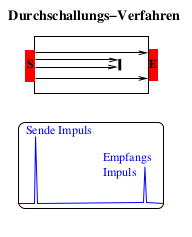
\includegraphics[height=6cm]{durch.png}
  \caption{Das Durchschallungsverfahren.}
  \label{fig:durch}
  \cite{skript}
\end{figure}

Der Sender sendet einen kurzzeitigen Schallimpuls aus, dieser wird am anderen Ende
der Probe durch den Empfänger aufgefangen. Falls sich Fehler oder Unebenheiten
in der Probe befinden, wird nur eine abgeschwächte Intensität am
Empfänger gemessen. Es ist keine Aussage über die Lage der Fehlerstelle
möglich.

\subsubsection{Impuls-Echo-Verfahren}
Bei diesem Verfahren, welches in Abbildung \ref{fig:echo}
dargestellt ist, fungiert der Ultraschallsender auch als Empfänger.

\begin{figure}[H]
  \centering
  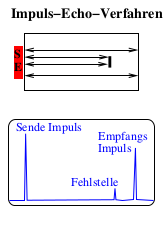
\includegraphics[height=6cm]{echo.png}
  \caption{Das Impuls-Echo-Verfahren}
  \label{fig:echo}
  \cite{skript}
\end{figure}

Der ausgesendete Impuls wird an einer Grenzfläche reflektiert und nach seiner
Rückkehr vom Empfänger registriert. Ist die Schallgeschwindigkeit
konstant kann über die Laufzeit $t$ die Lage der Fehlstelle über
\begin{equation}
  s=\frac{1}{2}ct
  \label{strecke}
\end{equation}
bestimmt werden. Sind Fehlerstellen vorhanden, dann kann die Höhe des
Echos Informationen über die Größe der Fehlstelle liefern.


\subsection{Vorbereitung}
Zur Vorbereitung auf den Versuch wurden materialspeziefische Werte recherchiert, diese
sind in Tabelle \ref{tab:tab1} gezeigt.

\begin{table}[H]
  \centering
  \caption{Werte für die Schallgeschwindigkeit.}
  \label{tab:tab1}
    \begin{tabular}{c |c c c}
    \toprule
    & Luft & dest. Wsser& Acryl\\
    \midrule
    Schallgeschwindigkeit c in m/s & 330 & 1480 & 2730\\
    \bottomrule
    \end{tabular}
    \cite{olympus}, \cite{halle}
  \end{table}

